\documentclass{standalone}
\usepackage[utf8]{inputenc}
\usepackage{newtxtext}
\usepackage{newtxmath}
\usepackage[italic]{hepnicenames}
\makeatletter\def\@shiftlen@anti@gen@bar{0mu}\makeatother
\usepackage[svgnames]{xcolor}
\usepackage{tikz-feynhand}


\begin{document}
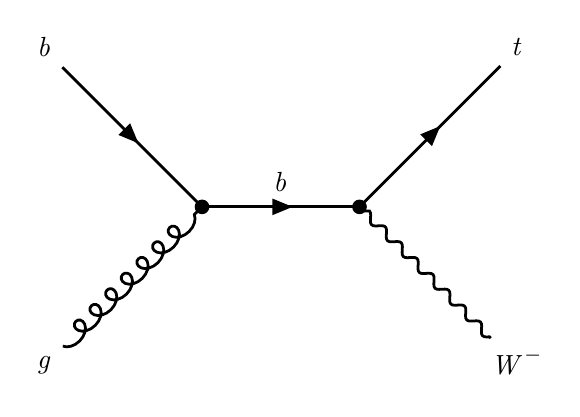
\begin{tikzpicture}
  \setlength{\feynhandlinesize}{1.0pt}
  \tikzfeynhandset{every dot={/tikz/color=Black},}
  \begin{feynhand}
    \vertex [particle, Black] (b) at (-3.0, 2.0) {\Pqb};
    \vertex [particle, Black] (g) at (-3.0, -2.0) {\Pg};
    \vertex [particle, Black] (t1) at (3.0, 2.0) {\Pqt};
    \vertex [particle, Black] (W) at (3.0, -2.0) {$\PW^-$};
    
    \vertex [dot, Black] (bg) at (-1.0, 0.0) {};
    \vertex [dot, Black] (tW) at (1.0, 0.0) {};
    
    \propagator [gluon, Black] (g) to (bg);
    \propagator [fermion, Black] (b) to (bg);
    \propagator [fermion, Black] (bg) to [edge label=\Pqb, color=Black] (tW);
    \propagator [fermion, Black] (tW) to (t1);
    \propagator [boson, Black] (W) to (tW);
  \end{feynhand}
\end{tikzpicture}
\end{document}
